\section{Method}
The hardware in this research project will be two different Raspberry PI's (model 1B and 3) that will be running one and one. the PI's is not going to work together. The same device will be hosting both the client and the server. and then controlled from a "master" computer.
For the software the \textit{C++ Based OPC UA Client \& Server SDK} \cite{opcSdk} will be used. To simulate different machines on the same device Doker \cite{docker} will be used where the client will be running in one container and the server in another.
Matlab will be used to analyce and plot the result from the measurements.

\bigskip

To answer the research questions mentioned in \cref{researchQuestion} the client will be triggered to ask the server for a specific size and type of data. The time from the moment the client ask's the server until it's received will be measured and analyzed. 
Different data sizes will be asked from the server to see if the access time get's affected. Matlab will then be used to plot the result. \cref{opcFlow} show an simplyfied image of this.


\begin{figure}[h]
    \centering
    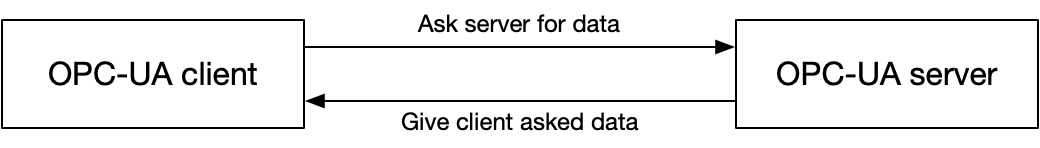
\includegraphics[width=1\textwidth]{./images/opcQuestion.png}
    \caption{client ask server for data} \label{opcFlow}
\end{figure}
